\chapter{Event Reconstruction}

In this chapter, the procedure for event reconstruction of the $B$ meson decay $B \to K K \ell \nu$ is shown, starting with final state particle selection and then combining them to obtain the $B$ meson candidates.

\section{Final State Particles Selection}
The Belle detector is not able to detect all kinds of particles. Neutrinos are one such example, since they escapes detection, therefore we can only reconstruct the charged tracks in the decay, which are the two charged kaons ($K$) and the light lepton ($e$ or $\mu$). These are some of the particles which are commonly referred to as the final state particles (FSP). Final state particles have a long lifetime and are usually the particles that we detect when they interact with the material in the detector.

At this point in the analysis, we do not apply any specific particle selections yet, which results in a large number of available particles and their combinations, and, consequently, the computation time. In order to minimize this effect, we perform this part of the study on a smaller subset of the available generic MC, experiments no. $23$ and $31$, which correspond to an integrated luminosity of $6.273\e{fb^{-1}}$ and $17.725\e{fb^{-1}}$, respectively. We chose these two experiments to approximate the appropriate ratio of SVD1 and SVD2 data in the full Belle MC.

\subsubsection{Leptons}

Figures \ref{fig:evars} and \ref{fig:muvars} show the impact parameters $d_0$ and $z_0$, the momentum in  $\Upsilon(4S)$ center-of-mass system (CMS), and the PID information for true and fake electrons and muons from any source, where true electrons/muons from the signal $B$ meson decay are shown separately. \textit{True} and \textit{fake} implies that the particles are correctly or wrongly reconstructed, with respect to the generated MC truth. The difference between the true leptons from any source and those from signal decays is due to the distinct kinematics of the parent's decay.

\begin{figure}[H]
	\centering
	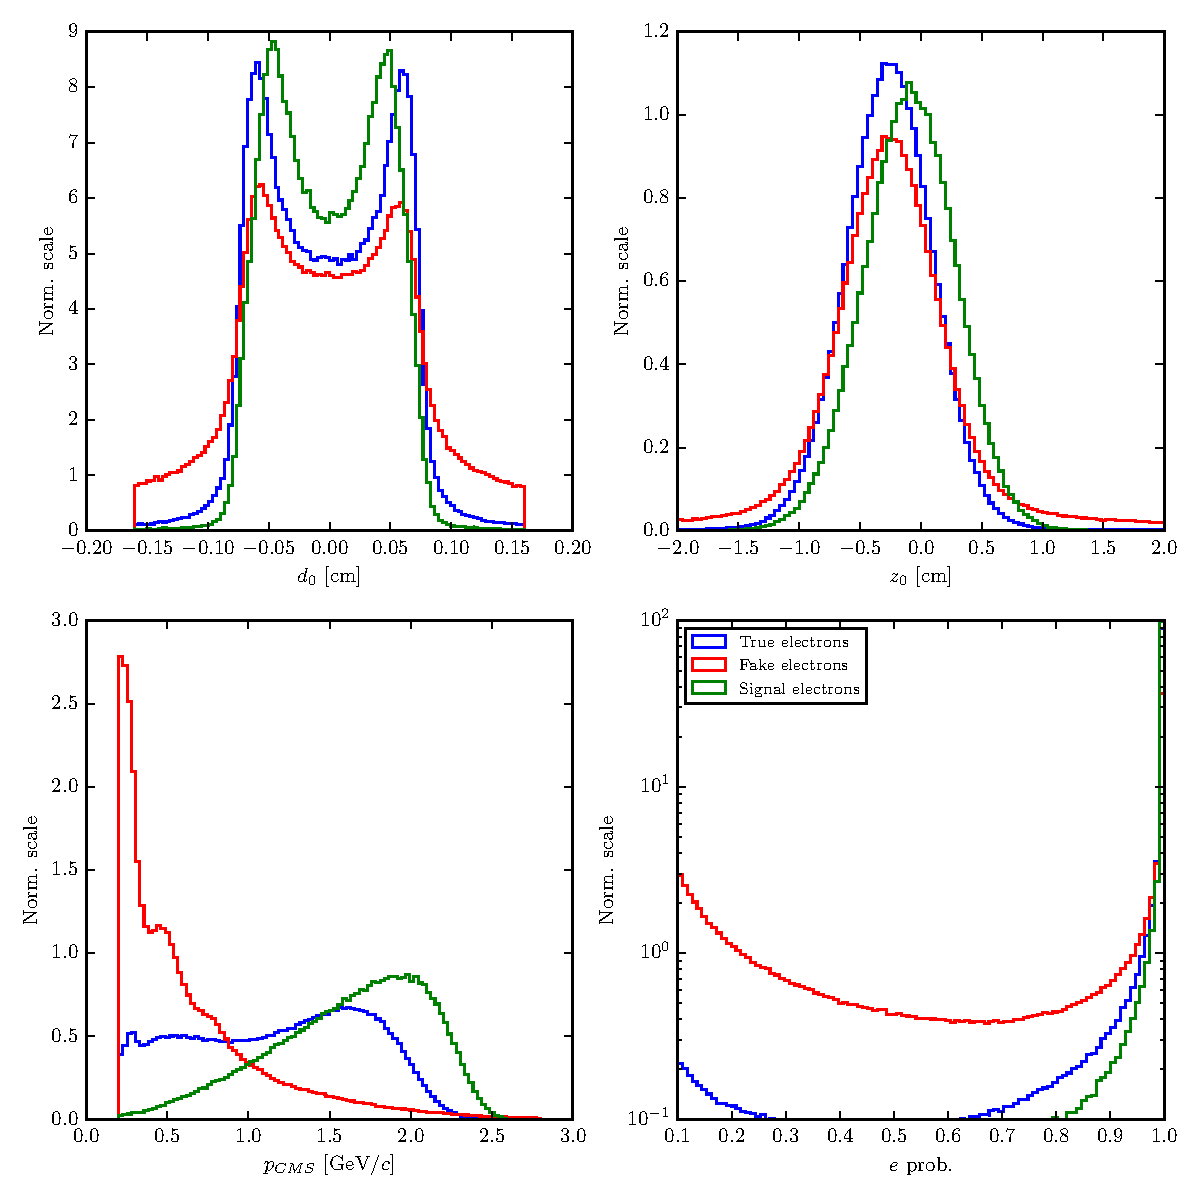
\includegraphics[width=\linewidth]{fig/FSP_e_vars}
	\captionsetup{width=.8\linewidth}
	\caption{Normalized properties of true (blue), fake (red) electrons from any source, and true electrons from signal $B$ candidates (green).}
	\label{fig:evars}
\end{figure}

\begin{figure}[H]
	\centering
	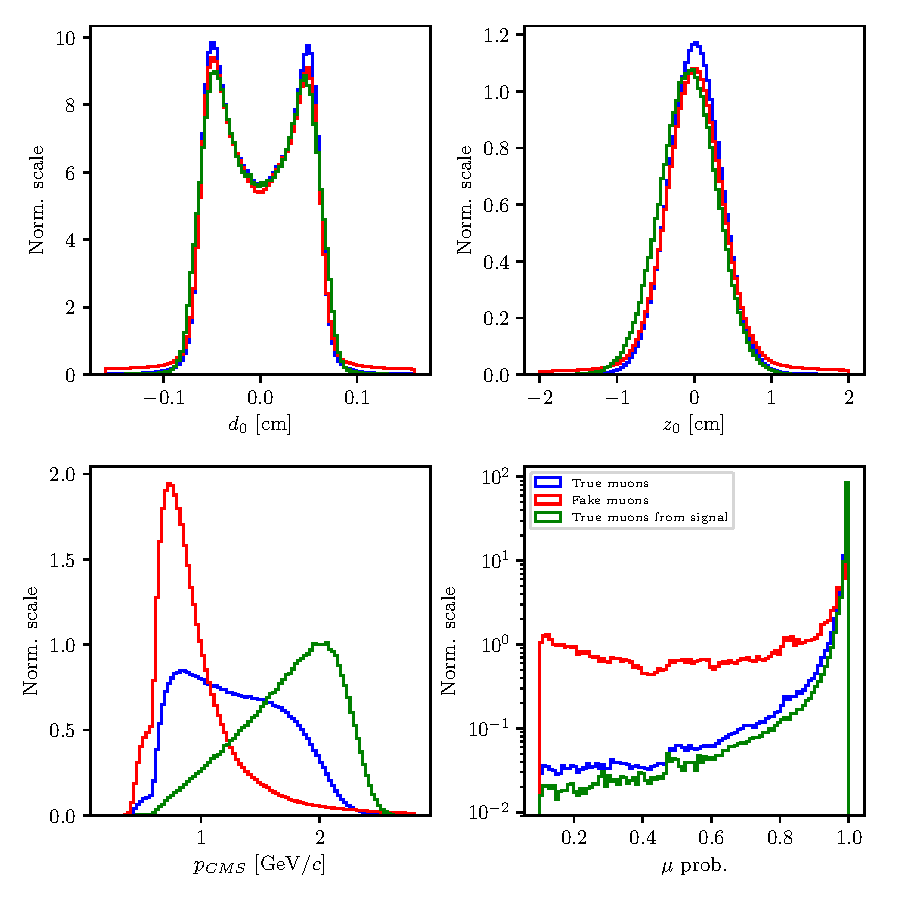
\includegraphics[width=\linewidth]{fig/FSP_mu_vars}
	\captionsetup{width=.8\linewidth}
	\caption{Normalized properties of true (blue), fake (red) muons from any source, and true muons from signal $B$ candidates (green).}
	\label{fig:muvars}
\end{figure}

Based on these distributions, we can define a selection criteria
\begin{itemize}
	\item $\vert d_0 \vert < 0.1\e{cm}$,
	\item $\vert z_0 \vert < 1.5\e{cm}$,
	\item $p_{CMS} \in [0.4,\,2.6]~\e{GeV}/c$ for electrons,
	\item $p_{CMS} \in [0.6,\,2.6]~\e{GeV}/c$ for muons.
\end{itemize}

After this we can determine the optimal PID selection for electrons and muons, where we optimize the criteria by maximizing the standard definition of \textit{figure of merit} ($FOM$), defined in Eq. (\ref{eq:fom})
\begin{equation}
\label{eq:fom}
FOM = \sqrt{\mathcal{E}\mathcal{P}} \propto \frac{S}{\sqrt{S+B}},
\end{equation} 
where the argument in the square root is the product of the efficiency ($\mathcal{E}$) and the purity ($\mathcal{P}$). The definitions of signal ($S$) and background ($B$) are somewhat fluid throughout the analysis and need to be defined for each $FOM$ separately. In this section we define two representations of $S$ and $B$. In $FOM_1$ the signal $S$ represents correctly reconstructed final state particles, while in $FOM_2$ the signal $S$ represents correctly reconstructed final state particles coming from correctly reconstructed $B$ meson candidates. In both cases the background represents all other particle candidates which do not satisfy the conditions of $S$.

The $FOM$ plots are shown in Figures \ref{fig:efom} and \ref{fig:mufom}. The selection criteria are based on PID cuts used for PID efficiency calibration. The optimal value for the PID cuts is equal to the largest available value for true leptons ($FOM_1$), as well as for true leptons from signal $B$ decays ($FOM_2$), so selections via both methods are the same. The optimal PID selection criteria for leptons are then
\begin{itemize}
	\item $e$ prob. $ > 0.9$ for electrons,
	\item $\mu$ prob. $ > 0.97$ for muons.
\end{itemize}

\begin{figure}[H]
	\centering
	\captionsetup{width=.8\linewidth}
	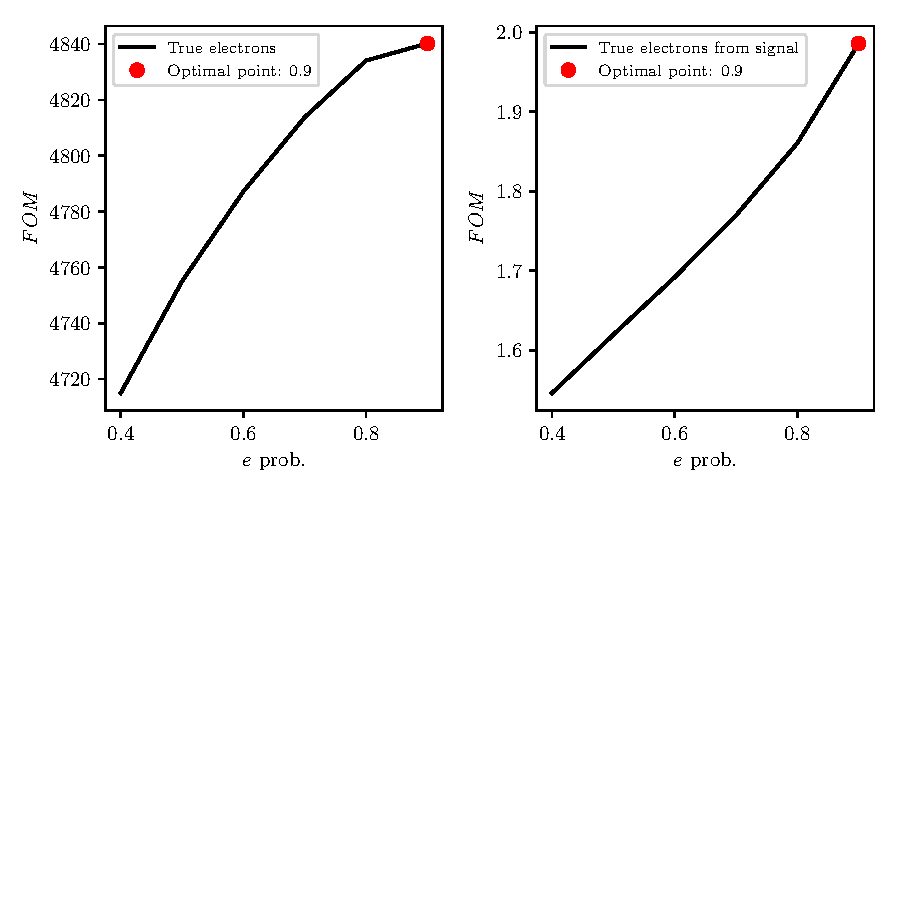
\includegraphics[width=\linewidth]{fig/FSP_e_fom}
	\caption{$FOM$ optimizations of the PID selection for true electrons (left) and true electrons from signal $B$ candidatess (right).}
	\label{fig:efom}
\end{figure}

\begin{figure}[H]
	\centering
	\captionsetup{width=.8\linewidth}
	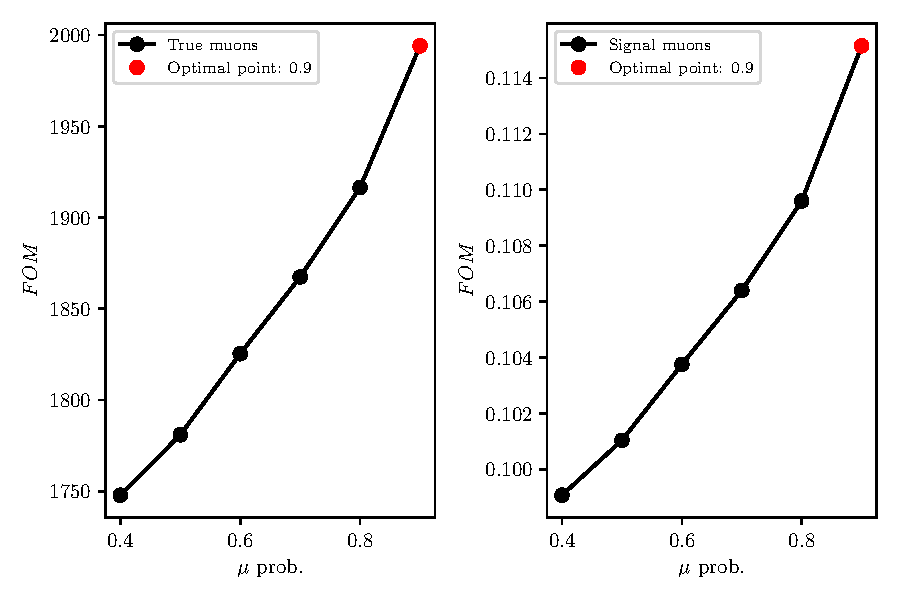
\includegraphics[width=\linewidth]{fig/FSP_mu_fom}
	\caption{$FOM$ optimizations of the PID selection for true muons (left) and true muons from signal $B$ candidates (right).}
	\label{fig:mufom}
\end{figure}


\subsubsection{Kaons}

We repeat the procedure for both kaons. Figure \ref{fig:Kvars} shows the impact parameters $d_0$ and $z_0$, the momentum in  $\Upsilon(4S)$ center-of-mass system (CMS), and the PID information for true and fake kaons, where true kaons from the signal decay are shown separately.

\begin{figure}[H]
	\centering
	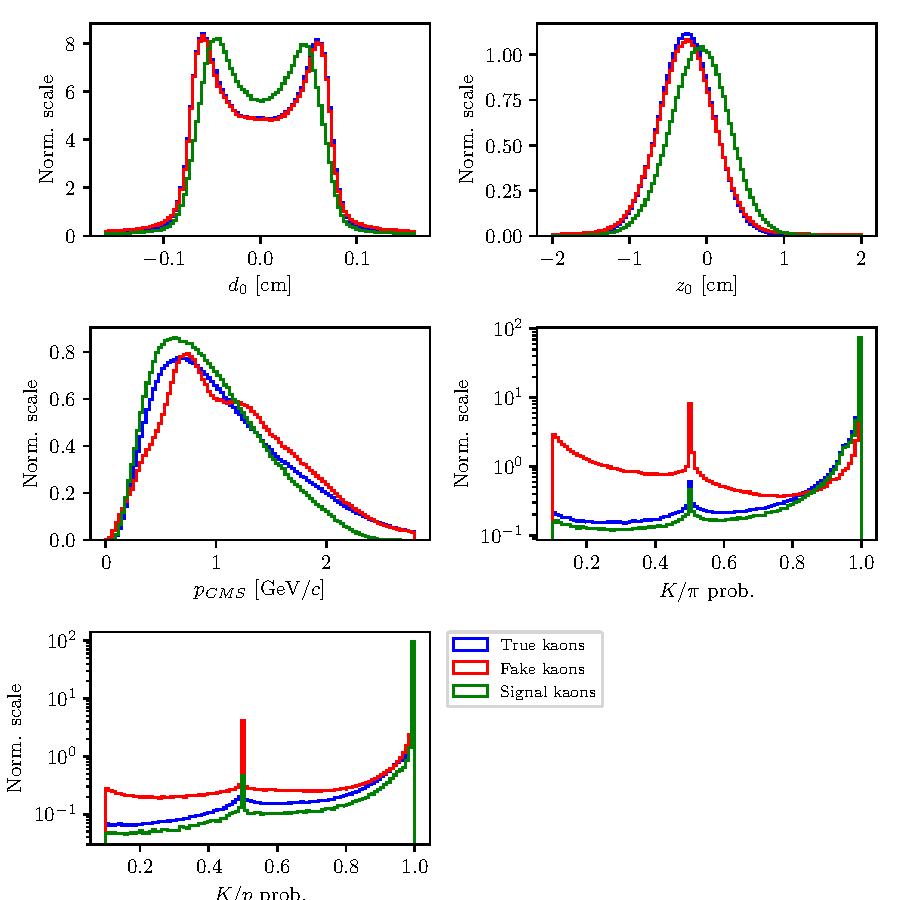
\includegraphics[width=\linewidth]{fig/FSP_kaon_vars}
	\captionsetup{width=.8\linewidth}
	\caption{Normalized properties of true (blue), fake (red) and true kaons (green) from signal $B$ candidates.}
	\label{fig:Kvars}
\end{figure}

We define the kaon selection criteria in the same manner as in the case for leptons
\begin{itemize}
	\item $\vert d_0 \vert < 0.15\e{cm}$,
	\item $\vert z_0 \vert < 1.5\e{cm}$,
	\item $p_{CMS} \in [0,\,2.5]~\e{GeV}/c$.
\end{itemize}

The PID optimization, in this case, is taken in two steps. First, we optimize the selection on $K / \pi$, and after that, the $K/p$ separation probability. Figure \ref{fig:Kfom} shows the optimization procedure for PID cuts on kaon candidates.

\begin{figure}[H]
	\centering
	\captionsetup{width=.8\linewidth}
	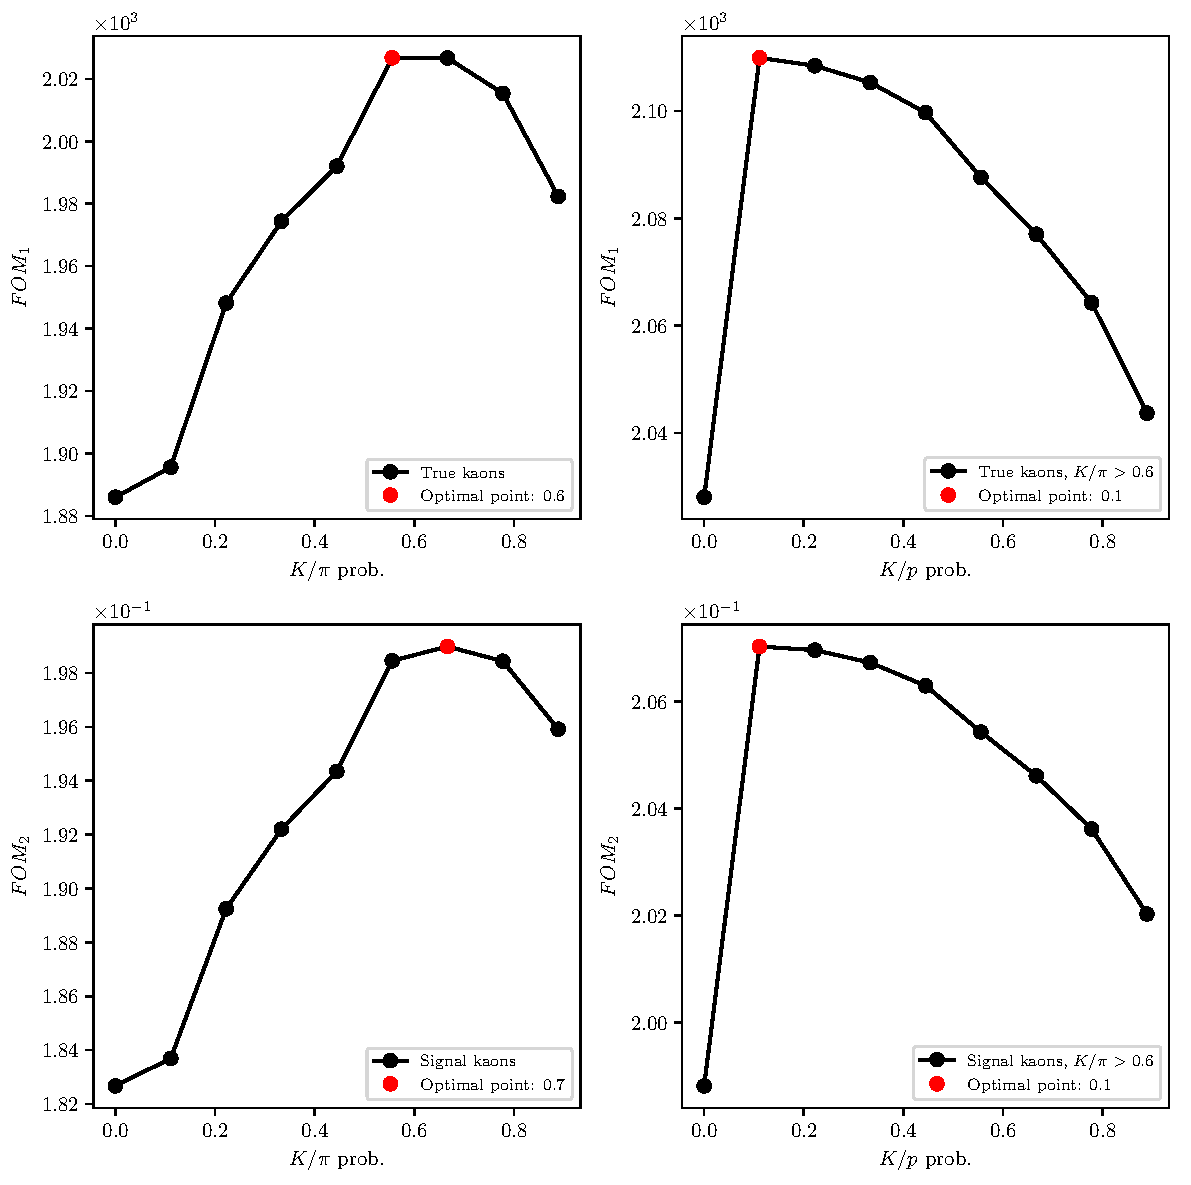
\includegraphics[width=\linewidth]{fig/FSP_kaon_fom}
	\caption{$FOM$ optimizations of the PID selection for true kaons (top) and true kaons from signal $B$ candidates (bottom). The plots on the left show the optimization of the first step for the $K / \pi$ probability cut, and the plot on the right the $K/p$ probability cut.}
	\label{fig:Kfom}
\end{figure}

The optimal PID selection for kaons is
\begin{itemize}
	\item $K/\pi > 0.6$,
	\item $K/p > 0.1$.
\end{itemize}

\section{Pre-selection of First \texorpdfstring{$B$}{B} Meson Candidates}

In this section, we use the charged particle candidates from the previous section to make particle combinations, which correspond to $B$ meson candidates. When a $B$ meson candidate is selected, additional features can be calculated and used for background rejection. Since we are still performing this part of the study on a smaller subset of the full available MC sample, we will perform an under-optimized selection based on the $FOM$ optimizations, in order to optimize them later on the full Belle MC sample.

Since the missing neutrino escapes detection, we reconstruct the $B$ mesons using the following final state particles
\begin{align*}
B^+ &\to K^+ K^- e^+, \\
B^+ &\to K^+ K^- \mu^+,
\end{align*}
and similarly for $B^-$. When an arbitrary combination is obtained, we perform a vertex fit of the three tracks in order to discard combinations with a low probability of tracks coming from the same point. $B$ mesons have a relatively long lifetime and decay along the $z$ axis of the detector in the direction of the boost, so the vertex fit is enforced with an \texttt{IPTUBE} constraint, which constrains the vertex to an elongated ellipsoid along the beam direction. We require that the fit converged and apply a selection on the minimal fit probability. The fit probability for signal and background $B$ meson candidates is shown in Figure \ref{fig:vtx} (left). We perform an $FOM$ optimization of this selection, which is shown in Figure \ref{fig:vtx} (right) for the subset of the Belle MC sample. In this, and in the following cases, the definition of $S$ from Eq. (\ref{eq:fom}) are correctly reconstructed $B$ meson candidates with a missing neutrino which are not coming from a $b \to c$ transition.

\begin{figure}[H]
	\centering
	\captionsetup{width=0.8\linewidth}
	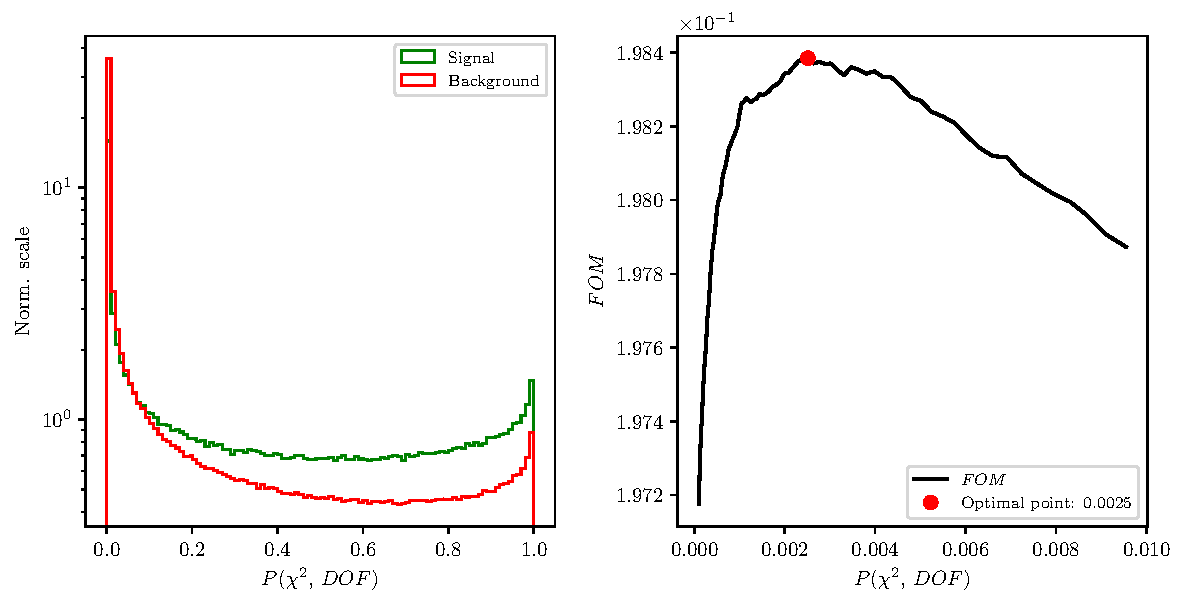
\includegraphics[width=\linewidth]{fig/VTX}
	\caption{Normalized vertex fit probability distribution for signal and background $B$ meson candidates in the logarithmic scale (left) and the $FOM$ optimization of the vertex fit probability (right) for the subset of the full Belle MC sample.}
	\label{fig:vtx}
\end{figure}

The chosen pre-selection on the fit probability is
\begin{itemize}
	\item $P(\chi^2,NDF) > 1.0\E{-3}$.

\end{itemize}

With the neutrino being the only missing particle on the reconstructed side, it is possible to determine the angle between the direction of the reconstructed $B$ (denoted as $Y \to K K \ell$) and the nominal $B$, as

\begin{align}
\mathrm{p}_\nu &= \mathrm{p}_B - \mathrm{p}_{Y}, \\
\label{eq:massnu}
\mathrm{p}_\nu^2 = m_\nu^2 &= m_B^2 + m_Y^2 - 2E_BE_Y + 2\vec{p}_B \cdot \vec{p}_Y \approx 0, \\ 
\label{eq:cosby}
\cos \left(\theta_{BY}\right) &= \frac{2E_BE_Y - m_B^2 - m_Y^2}{2\vert \vec{p}_B \vert \vert \vec{p}_Y\vert},
\end{align} 

where $p$ denotes a scalar, $\vec{p}$ a vector, and $\mathrm{p}$ a four-vector. All the energy and momenta above are calculated in the CMS frame. The mass of the neutrino is equal to 0 up to a very good precision, so we use it in Eq. (\ref{eq:massnu}). Additionally, we substitute the unknown energy and momentum magnitude, $E_B$ and $\vert \vec{p}_B \vert$, of the $B$ meson in Eq. (\ref{eq:cosby}), with quantities from the well known initial conditions
\begin{align}
E_B &= E_{CMS} / 2,\\
\vert \vec{p}_B \vert = p_B &= \sqrt{E_B^2 - m_B^2},
\end{align} 

where $E_{CMS}$ is the total energy of the $e^+e^-$ collision in the CMS frame and $m_B$ is the nominal mass of the $B$ meson. This improves the resolution of $\cos \left(\theta_{BY}\right)$, which leads to better signal-to-background discrimination.

For the correctly reconstructed candidates, this variable lies in the $[-1,1]$ region, though only to a certain precision, due to the finite detector resolution. Background candidates, however, populate also the non-physical regions, as shown in Figure \ref{fig:cosby} (left). 

\begin{figure}[H]
	\centering
	\captionsetup{width=.8\linewidth}
	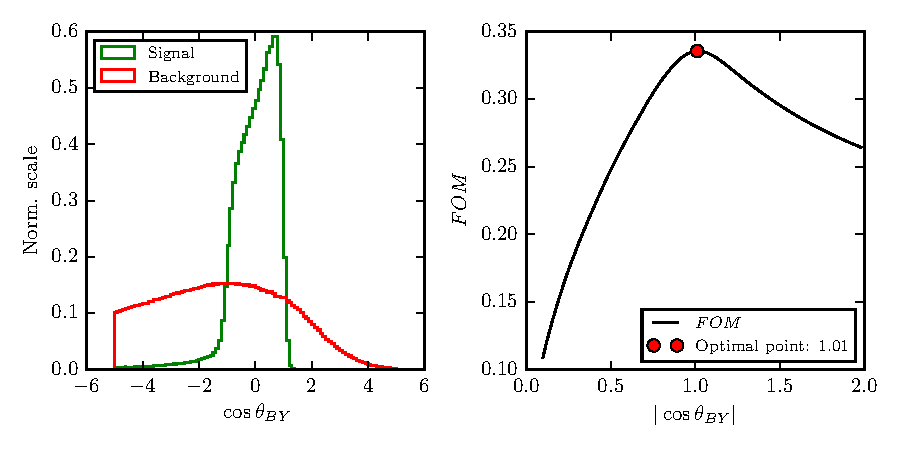
\includegraphics[width=\linewidth]{fig/cosBY}
	\caption{The normalized $\cos \theta_{BY}$ distribution for signal and background $B$ meson candidates (left) and the $FOM$ optimization of the $\cos \theta_{BY}$ variable (right) for the subset of the full Belle MC.}
	\label{fig:cosby}
\end{figure}

We again impose an under-optimized selection on this variable from Figure \ref{fig:cosby} (right) to discard a large amount of background on this subset of the full Belle MC
\begin{itemize}
	\item $\vert \cos \left(\theta_{BY}\right) \vert < 1.20$.
\end{itemize}

\section{Loose Neutrino Reconstruction}\label{sec:loose-neutrino-reconstruction}
We are not able to directly determine the four-momentum of the missing neutrino. However, due to the detectors geometry, which almost completely covers the full solid angle, and due to the well known initial conditions of the $\Upsilon(4S)$ meson, it is possible to determine the kinematics of the missing neutrino indirectly. Specifically, this is performed by reconstructing the companion $B$ meson via summing up the four-momenta of all the FSP particles in the event, which were not used in the reconstruction of the signal side $B$ meson. This is known as the \textit{untagged} method, since we are not using any kind of tagging method to reconstruct the companion $B$ meson. The particles used in the indirect companion $B$ meson reconstruction are also said to belong to the \textit{rest of the event} (ROE).

Due to the beam background in the detector, material interactions, or other processes, random tracks and clusters enter our event and get reconstructed as part of the physics process we want to study. In order to remedy this, we perform an extensive clean-up of the tracks and clusters in the ROE side before calculating the four-momentum of the missing part of the event. The clean-up procedure is performed separately on tracks and clusters, and uses multiple steps with multivariate analysis (MVA) algorithms in order to separate good tracks and clusters from the background ones, which also populate the ROE. Then, for each ROE object, a ROE mask is created for tracks and clusters, which narrates the use of this object in the final calculations of the ROE four-momentum. From this point on, we assume the ROE to be efficiently cleansed of extra tracks and clusters. A more detailed description of the ROE clean-up can be found in Chapter \ref{sec:roe}. 

The total missing four-momentum in the event can be determined as
\begin{align}
\mathrm{p}_{miss} &= \mathrm{p}_{\Upsilon(4S)} - \sum_i^{\mathrm{Event}}\left(E_i,\,\vec{p}_i \right),\\
\label{eq:ROEloop}
\mathrm{p}_{miss} &= \mathrm{p}_{\Upsilon(4S)} - \left(\mathrm{p}_{Y} -\sum_i^{\mathrm{Rest~of~event}}\left(E_i,\,\vec{p}_i \right)\right),
\end{align}

where the summation runs over all charged and neutral particles in the defined set with
\begin{equation}
\mathrm{p}^{\mathrm{neutral}}_i = \left(p_i,\, \vec{p}_i \right) \quad \mathrm{and} \quad \mathrm{p}^{\mathrm{charged}}_i = \left(\sqrt{m_i^2 + p_i^2},\, \vec{p}_i \right)
\label{eq:pcharged}
\end{equation}
We assume all neutral particles to be massless. For charged tracks in the ROE, a mass hypothesis needs to be defined in order to determine the energy of the track. After the ROE clean-up, we make the following procedure of choosing the mass hypothesis
\begin{enumerate}
	\item $e$, if $e$ prob. $> \mu$ prob. and $e$ prob. $> 0.9$,
	\item otherwise $\mu$, if $\mu$ prob. $> e$ prob. and $\mu$ prob. $> 0.97$,
	\item otherwise $K$, if $K/\pi$ prob. $> 0.6$,
	\item otherwise $\pi$.
\end{enumerate} 
We calculate the square of the missing mass, $m_{miss}^2$, which is consistent with zero, if signal-side neutrino is the only missing particle in the event. The $m_{miss}^2$ distribution is shown in Eq. (\ref{eq:m2def}).
\begin{align}
\label{eq:nuold}
\mathrm{p}_\nu &= \mathrm{p}_{miss} = \left(E_{miss},\,\vec{p}_{miss} \right),\\
\label{eq:m2def}
m_{miss}^2 &= \mathrm{p}_{miss}^2 = \mathrm{p}_{\nu}^2 = m_\nu^2 \approx 0.
\end{align}

Since the detector performance is not perfect, the distribution of the $m_{miss}^2$ variable has a non-zero width. Additionally, a tail is introduced due to missing particles like neutrinos, other neutral undetected particles such as $K_L^0$, or simply missing tracks, due to detection failure. Figure \ref{fig:missm2} shows the distribution of $m_{miss}^2$, as defined with the missing four-momentum in Eq. (\ref{eq:nuold}). Correctly reconstructed candidates, which come from events, where the other $B$ meson decayed via a hadronic decay mode, peak at zero. If the companion $B$ meson decayed (semi-)leptonically, candidates are shifted to larger values of this variable, even if the event in question is a signal event. For this purpose, we define a subset of all signal candidates, which come from events where the companion $B$ meson decayed hadronically and all of its particles were taken into account correctly. We only allow for missing photons, since they are frequently radiated due to bremsstrahlung effects from final-state electrons and they typically do not have a big impact on the four-momentum of the final candidate. We denote this subset as the \textit{perfect} signal. This subset is used to correctly define the clean-up parameters and is not used in any reconstruction steps, since we cannot know in data which neutral particles are actually missing.

Due to this fact, we impose a selection on the $m_{miss}^2$ variable, in order to partially discard candidates with spoiled properties, even if it was in principle a correct combination of FSP particles on the signal side. The selection was chosen based on the optimization of the $FOM$, where in this case the definition of $S$ were perfectly reconstructed signal candidates. The chosen selection is 
\begin{itemize}
	\item $\vert m_{miss}^2 \vert < 3.0\e{GeV}/c^2$,
\end{itemize}
which is also under-optimized at this point, due to the same reasons as in the cases above.


\begin{figure}[H]
	\centering
	\captionsetup{width=.8\linewidth}
	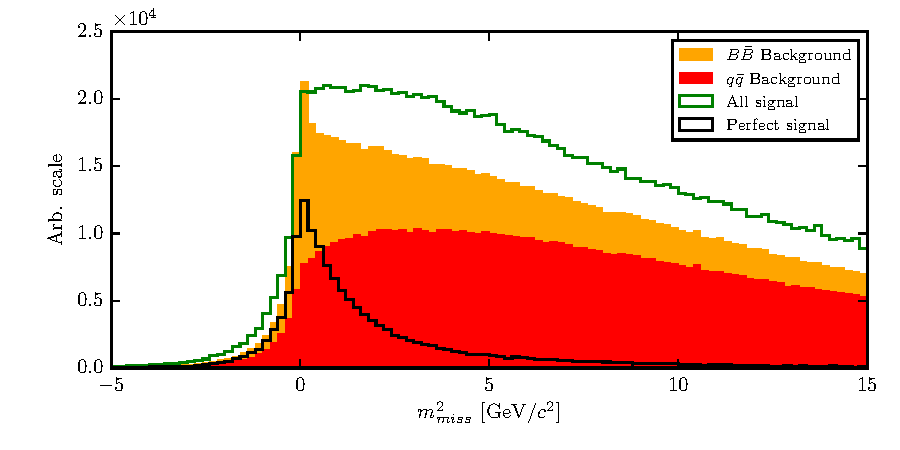
\includegraphics[width=\linewidth]{fig/missM2}
	\caption{$m_{miss}^2$ distribution for signal and various types of background. All signal (green) and perfect signal (black) are scaled up equally.}
	\label{fig:missm2}
\end{figure}

The main uncertainty of the neutrino four-momentum, defined in Eq. (\ref{eq:nuold}), comes from the energy uncertainty. It is a common practice to substitute the missing energy with the magnitude of the missing momentum, since the momentum resolution from the measurement is much better,
\begin{equation}
\label{eq:nunew}
\mathrm{p}_\nu = \left(\vert \vec{p}_{miss} \vert,\,\vec{p}_{miss} \right).
\end{equation}
This also fixes the neutrino mass to $0\e{GeV}/c^2$. The newly defined neutrino four-momentum can be added to the four-momentum of the $Y(KK\ell)$ candidate to obtain the full $B$ meson four-momentum and calculate the traditional $M_{BC}$ and $\Delta E$ variables
\begin{align}
\label{eq:de}
\Delta E &= E_B - E_{CMS}/2,\\
M_{BC} &= \sqrt{\left(E_{CMS}/2\right)^2 - \vert \vec{p}_B \vert^2}.
\end{align}

Since the final fit will be performed over \vars, we define the fit region
\begin{itemize}
	\item $M_{BC} \in [5.1,\,5.295]\e{GeV}/c^2$,
	\item $\Delta E \in [-1.0,\,1.3]\e{GeV}$.
	%\item Signal enhanced region: $M_{BC} \in [5.27,\,5.295]\e{GeV}/c^2$ and $\vert \Delta E \vert < 0.143 \e{GeV}$,
\end{itemize}

Figure \ref{fig:mbc_de_pre} shows the distributions of $\Delta E$ (left) and $M_{BC}$ (right) for signal and major types of background after the pre-selection. Both signal components (all signal and perfect signal) are scaled up with respect to the background components but are in proper scale one to another. The effects of missing particles are clearly seen based on the shape difference between full and perfect signal.

\begin{figure}[H]
	\centering
	\captionsetup{width=0.8\linewidth}
	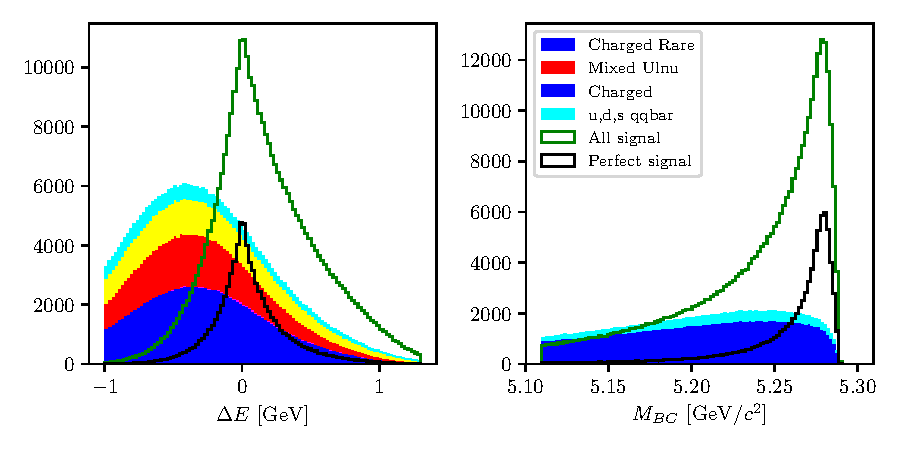
\includegraphics[width=\linewidth]{fig/mbc_de_pre}
	\caption{Distributions of $\Delta E$ (left) and $M_{BC}$ (right) for signal and major types of background after the pre-selection. Both signal components are scaled up with respect to the background components, but are in proper scale one to another. The perfect signal has a much better resolution in both distributions, since the event is perfectly reconstructed.}
	\label{fig:mbc_de_pre}
\end{figure}

\subsection{\texorpdfstring{$q^2$}{q2} calculation}
$q^2$ is the squared Lorentz invariant of the four-momentum, also known as \textit{momentum transfer squared}, which is transferred from the $B$ meson to the $W$ boson. There are several possible calculations of this variable which offer a different resolution. In this analysis, we follow the calculation procedure of $q^2$ from \cite{VubCLEO}, which yields the best resolution.

For correctly reconstructed events, Eq. (\ref{eq:de}) satisfies the condition $\Delta E \approx 0$ within precision. It is possible to rescale the neutrino energy in such way that we fix $\Delta E$ to zero, meaning 
\begin{equation}
\Delta E' = (E_Y + \alpha E_\nu) - E_{CMS}/2 = 0.
\end{equation}
and calculate a corrected value of $M_{BC}$
\begin{equation}
M_{BC}' = \sqrt{\left(E_{CMS}/2\right)^2 - \vert \vec{p}_Y + \alpha \vec{p}_\nu \vert^2}.
\end{equation}

The neutrino momentum resolution dominates the $\Delta E$ uncertainty, so the correction factor $\alpha$ reduces this effect.

A second correction can be applied by rotating the direction of the neutrino momentum by a small angle with respect to the reconstructed one. Such an angle is chosen in order fix the value of $M_{BC}'$ to the nominal mass of the $B$ meson, $m_B$.

The corrected neutrino momentum is then fixed to expected values of \vars, and is solely used for the $q^2$ calculation. With $\mathrm{p}_\ell$ as the reconstructed lepton four-momentum, we define the $q^2$ as
\begin{equation}
\label{eq:q2}
q^2 = \mathrm{q}^2 = \left(\mathrm{p}_\ell + \mathrm{p}_\nu \right)^2.
\end{equation}

The $q^2$ distributions and the corresponding resolutions are shown in Figure \ref{fig:q2}, along with other methods of $q^2$ determination.
\begin{figure}[H]
	\centering
	\captionsetup{width=0.8\linewidth}
	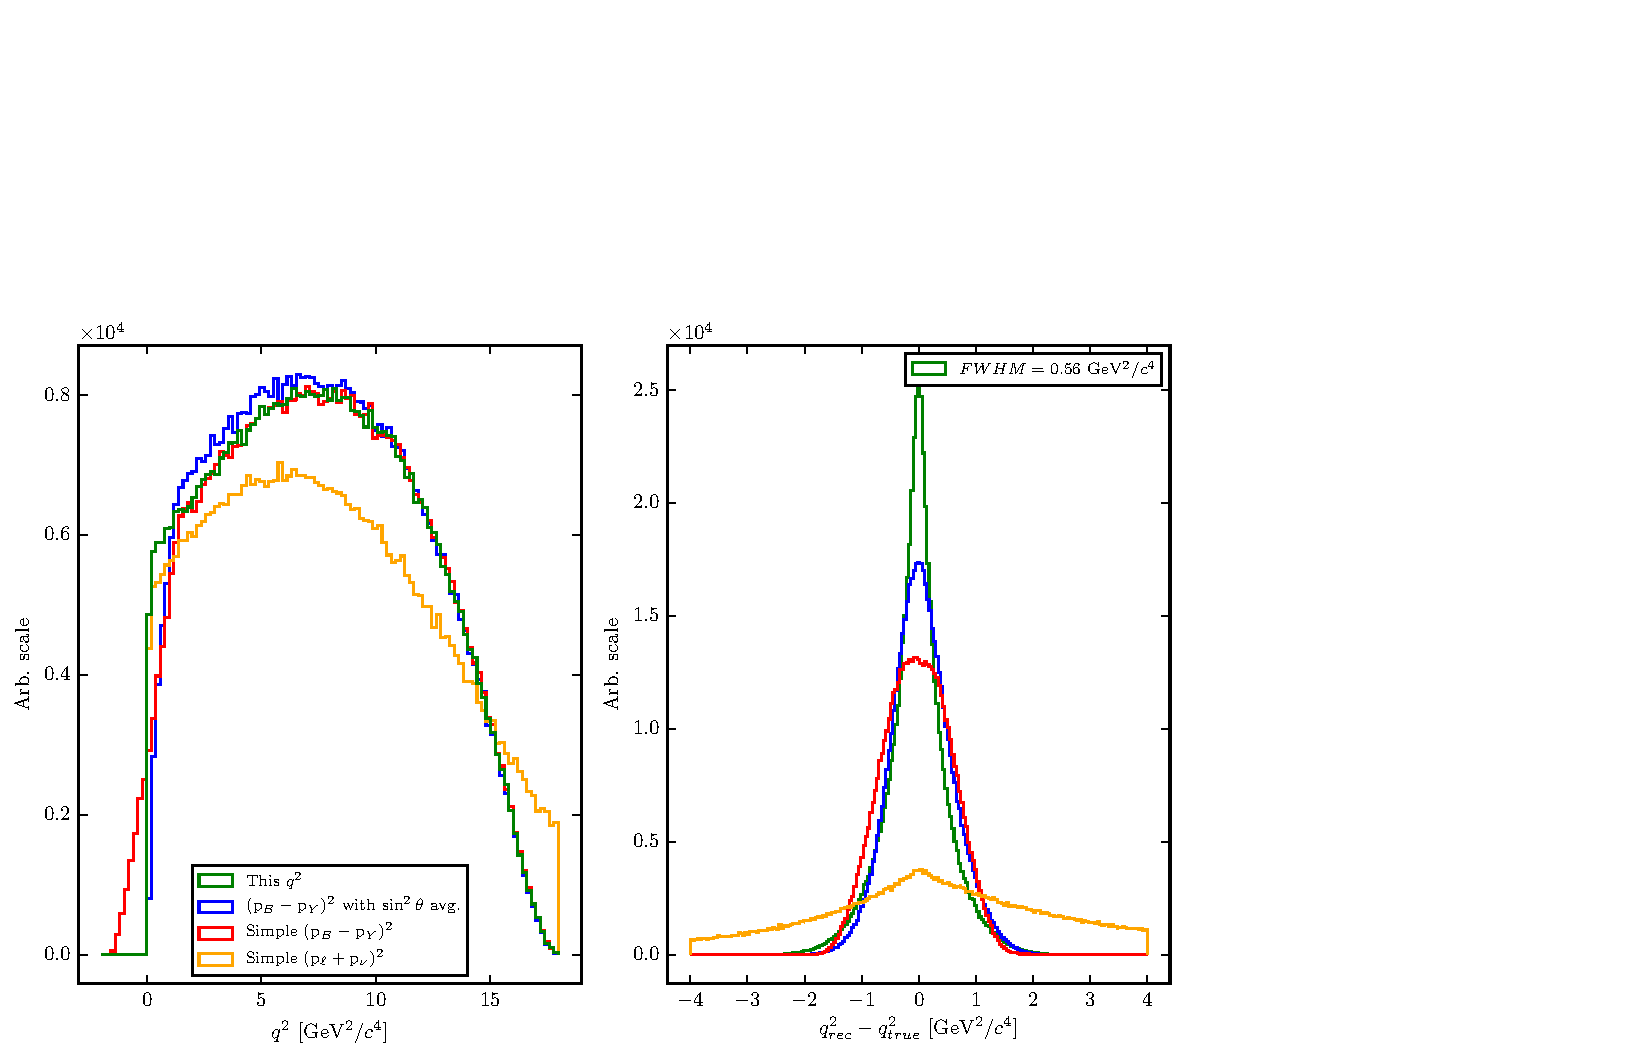
\includegraphics[width=\linewidth]{fig/q2}
	\caption{Distributions of $q^2$ (left) and $q^2$ resolution (right) for various methods of $q^2$ calculation. The green distribution follows the procedure in \cite{VubCLEO}, the blue distribution takes into account the weighted average of the $B$ meson direction \cite{Ha:2010rf}, and the red and orange distributions are straight-forward calculations with available information in the reconstruction. The $q^2$ calculation in red assumes a resting $B$ meson in the CMS frame, and the calculation in orange uses the neutrino four-momentum from Eq. (\ref{eq:nuold}).}
	\label{fig:q2}
\end{figure}

One must bear in mind that even though the chosen calculation yields the most precise result, this does not affect the correctness of the $q^2$ model, which was used in MC simulation (\texttt{ISGW2} \cite{Scora:1995ty}). Since the signal decay has not been observed yet, we do not have a good description of the decay model, and we treat this as a source of systematic uncertainty in this analysis.
\newpage
\section{Final Stage Optimization}

With the charge particle selection and a rough selection of the $B$ meson particles in place, we can now afford to run the reconstruction procedure over all of the $10$ streams of the full available Belle generic MC. After obtaining the full reconstructed sample, the first task is to optimize the under-optimized selection criteria from the previous stage. Repeating the procedure on the full sample results in the $FOM$ shapes shown in Figure \ref{fig:preciseFOM}, with the optimal selection criteria

\begin{itemize}
	\item $P(\chi^2,NDF) > 6.0\E{-3}$,
	\item $\vert \cos \left(\theta_{BY}\right) \vert < 1.05$.
\end{itemize}

\begin{figure}[H]
	\centering
	\captionsetup{width=0.8\linewidth}
	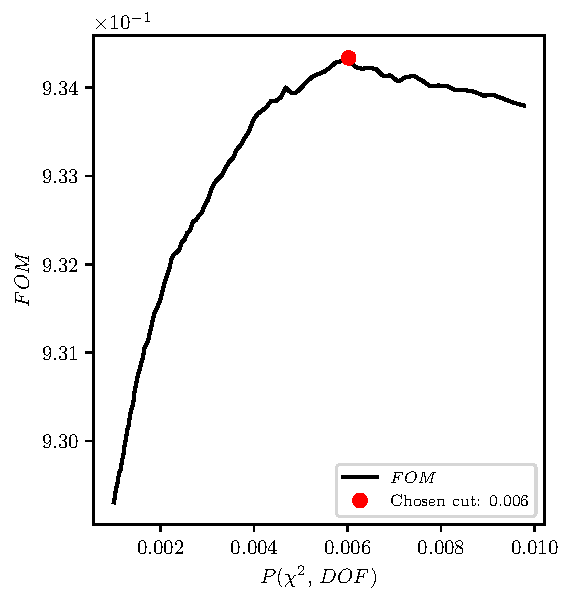
\includegraphics[width=0.48\linewidth]{fig/VTX_precise}
	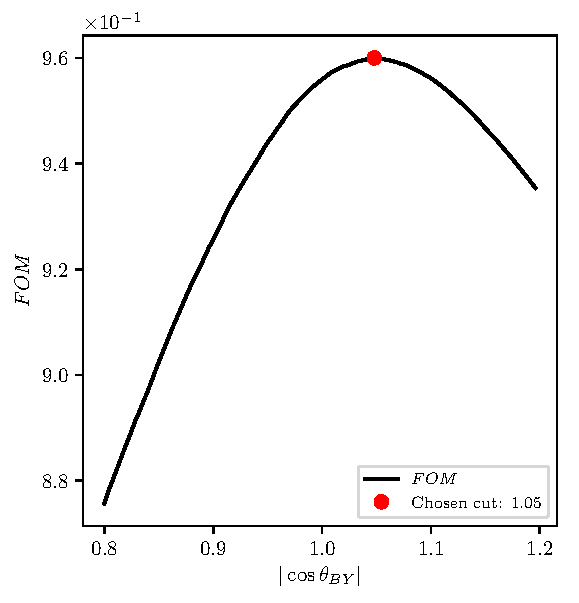
\includegraphics[width=0.48\linewidth]{fig/cosBY_precise}
	\caption{The $FOM$ optimization of the vertex fit probability (left) and the $\cos \theta_{BY}$ variable (right) for the full Belle MC sample.}
	\label{fig:preciseFOM}
\end{figure}

With further optimizations, we will be fine-tuning the signal-to-background ratio. The most prominent and distinguishable part of our signal is the perfect signal. For this purpose, we define a signal region in \vars, where most of our perfectly reconstructed candidates lie. We use this region for all of the following optimization steps in this chapter and also in the background suppression (Chapter \ref{sec:background-suppression}), since this allows us to better improve the signal-to-background ratio. The 2D $FOM$ optimization of the optimal \vars~signal region is shown in Figure \ref{fig:sigwin}.

The signal region is defined as
\begin{itemize}
	\item $M_{BC} > 5.271\e{GeV}/c^2$,
	\item $\vert \Delta E \vert < 0.126\e{Gev}$. 
\end{itemize}

\begin{figure}[H]
	\centering
	\captionsetup{width=0.8\linewidth}
	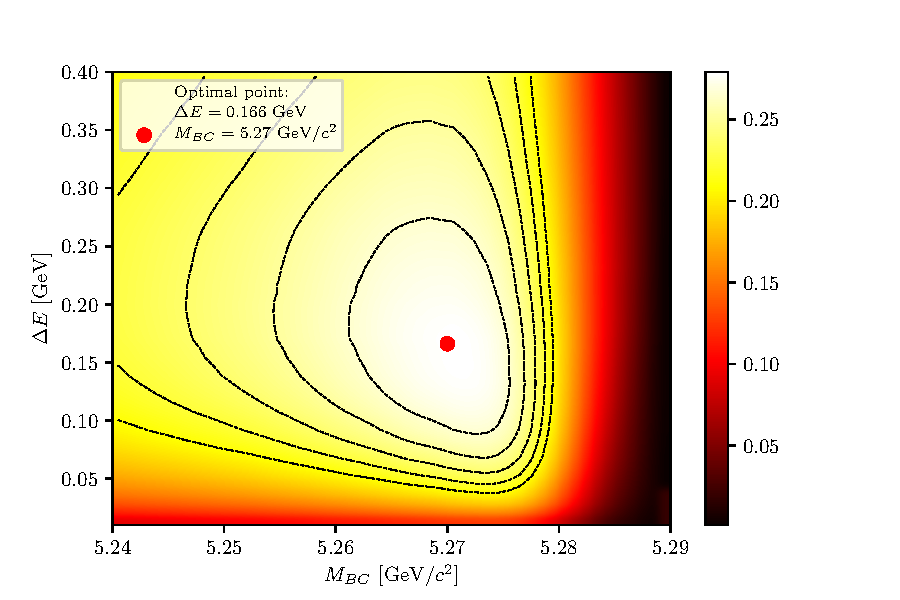
\includegraphics[width=\linewidth]{fig/sigWin}
	\caption{2D $FOM$ optimization of the signal region definition, where most of the perfectly reconstructed candidates are located.}
	\label{fig:sigwin}
\end{figure}

With the signal window defined, we can tighten the selection on $m_{miss}^2$, which we intentionally left loose before the signal categorization. With the $FOM$ optimization of perfectly reconstructed candidates inside the signal region, shown in Figure \ref{fig:missm2opt}, the optimal selection of $m_{miss}^2$ range is 

\begin{itemize}
	\item $\vert m_{miss}^2 \vert < 0.975\e{GeV}/c^2$.
\end{itemize}

\begin{figure}[H]
	\centering
	\captionsetup{width=0.8\linewidth}
	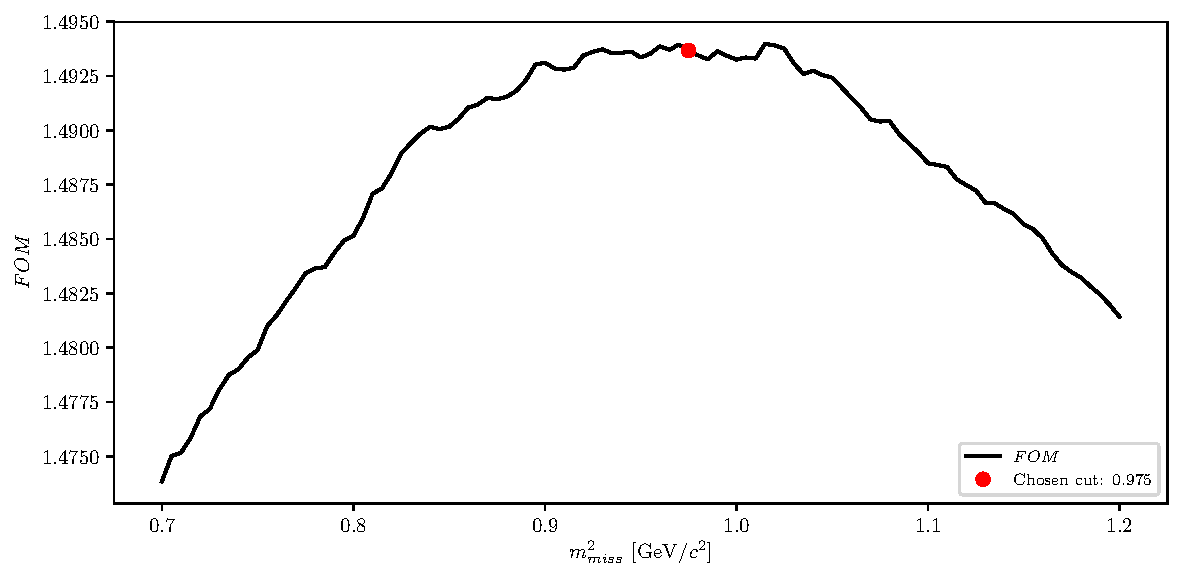
\includegraphics[width=\linewidth]{fig/missM2_precise}
	\caption{$FOM$ optimization of the $m_{miss}^2$ selection in the signal region.}
	\label{fig:missm2opt}
\end{figure}

\newpage
\section{Charge product categorization}\label{sec:event-categorization}

The missing information, due to an escaping neutrino in our reconstructed channel, is replaced by the information from the companion $B$ meson. Since this is an untagged reconstruction, the quality of the companion $B$ meson affects the properties of the signal candidate. Perfect reconstruction of a hadronically decayed companion $B$ meson results in pronounced peaks at $\Delta E \approx 0$, $m_{miss}^2 \approx 0$, and $M_{BC} \approx m_B$, while imperfect reconstruction, due to any kind of missing particles, produces tails, shift, or simply a worse resolution of the mentioned distributions. These effects are undesired, since they make it harder to separate signal from background.

To remedy this, we look at the charge product of the reconstructed $B$ meson and the ROE object. For correctly reconstructed events, this should have a value of 
\begin{equation}
\label{eq:chargeprod}
q_{B^\pm}q_{B^\mp} = -1,
\end{equation}

however, this value is distributed due to missing, or additional background charged particles in the ROE. Figure \ref{fig:sig_categ} shows various signal distributions of \vars~in arbitrary (left) and normalized (right) scales. We find the relative ratios of $67.86~\%$ and $32.14~\%$ for correct and wrong values of the charge product. Correctly reconstructed events represent the majority of the signal candidates and also have the best resolution in \vars, hence we proceed with the analysis by imposing the selection in Eq. \ref{eq:chargeprod}.

While this selection introduces a drop in the signal efficiency of about $32.14~\%$, it improves the resolution of our signal \vars~distributions and also the signal-to-background ratio, where the latter changes from $0.95\E{-3}$ to $1.09\E{-3}$.

\begin{figure}[H]
	\centering
	\captionsetup{width=0.8\linewidth}
	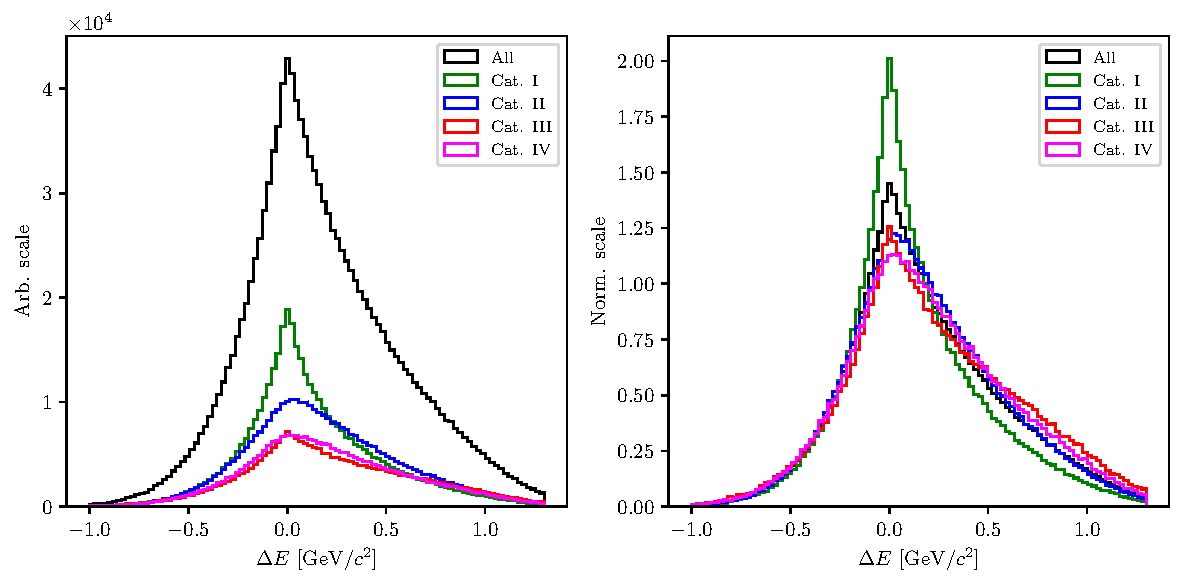
\includegraphics[width=\linewidth]{fig/sig_categ}
	\caption{Signal distributions of \vars~based on the charge product of both $B$ mesons in the event. The plots on the left show the distributions in an arbitrary scales, while the plots on the right show the normalized distributions.}
	\label{fig:sig_categ}
\end{figure}

\newpage
\section{Selection Summary}
\label{s:ss}
In this section, one can find the full summary of final selection criteria in the event reconstruction, from FSP particles up to the $B$ meson.

\begin{itemize}
	\item FSP particles:
	\begin{itemize}
		\item electrons: $\vert d_0 \vert < 0.1\e{cm},\,\vert z_0 \vert < 1,5\e{cm},\,p>0.6\e{GeV}/c,\\p_{CMS}\in[0.4,\,2.6]\e{GeV}/c,\,eID>0.9,$
		\item muons: $\vert d_0 \vert < 0.1\e{cm},\,\vert z_0 \vert < 1,5\e{cm},\,p_{CMS}\in[0.6,\,2.6]\e{GeV}/c,\\\mu ID>0.97,$
		\item kaons: $\vert d_0 \vert < 0.15\e{cm},\,\vert z_0 \vert < 1,5\e{cm},\,p_{CMS} < 2.5\e{GeV}/c,\\K/\pi~ID>0.6,\,K/p~ID>0.1,$
	\end{itemize}
	\item $B$ meson candidates:
	\begin{itemize}
		\item standard selection: $P(\chi^2,\,DOF) > 6\E{-3},\,\vert \cos \theta_{BY} \vert < 1.05,\,\vert m_{miss}^2\vert<0.975\e{GeV}/c^2,$
		\item fit region selection: $\Delta E \in [-1.0,1.3]\e{GeV},\,M_{BC} \in [5.1,5.295]\e{GeV}/c^2,$
		\item signal region selection: $\vert \Delta E \vert < 0.126\e{GeV},\,M_{BC} > 5.271\e{GeV}/c^2,$
		\item charge categorization: $q_{B^\pm}q_{B^\mp} = -1.$
	\end{itemize}
\end{itemize}